\documentclass[border=4pt,12pt]{standalone}
% House style for redrawn exam diagrams (diagram-v4: 0.4pt lines, filled -latex arrows, fine dashes; stipple and hatching drawn as real dots/lines (no PDF/SVG patterns, so they render in every browser and at any scale); transparent background). Every figure \input's this.
\usepackage{amsmath,amssymb}
\usepackage{txfonts}
\usepackage{pdfrender,xcolor}
% \halo{text}: label on shading. The shading stops just around each letter's outline (a thin knock-out that follows the
% glyphs, like the papers' typesetting), never a box. Owner: "I don't want a box around the text".
\newcommand{\halo}[1]{\leavevmode\rlap{\pdfrender{TextRenderingMode=2,LineWidth=2.2pt,LineJoinStyle=1,StrokeColor=white,FillColor=white}#1}#1}
\usepackage{tikz,pgfplots}
\pgfplotsset{compat=1.18}
\usetikzlibrary{arrows.meta,calc,angles,quotes,patterns,patterns.meta,intersections,positioning,decorations.markings,shapes.geometric}
% Stipple and hatching are drawn as actual dots / lines clipped to the region (path picture), NOT as pattern fills:
% SVG <pattern> fills vanish or blur when browsers scale the image, so the owner could not see the shading.
% Each dot is a 0.72pt square (keeps SVGs small; reads as a dot at print size). Dots sit on one global staggered grid, so neighbouring regions line up.
\makeatletter
\newdimen\ex@x \newdimen\ex@y \newdimen\ex@xa \newdimen\ex@ya \newdimen\ex@xb \newdimen\ex@yb \newcount\ex@row
\def\exam@stipplecolor{black!75}\def\exam@dotr{0.42pt}\def\exam@dotgap{2.5}
\def\ex@rowdots{\ifdim\ex@x<\ex@xb \pgfpathrectangle{\pgfqpoint{\dimexpr\ex@x-0.36pt\relax}{\dimexpr\ex@y-0.36pt\relax}}{\pgfqpoint{0.72pt}{0.72pt}}\advance\ex@x by \exam@dotgap pt\relax\expandafter\ex@rowdots\fi}
\def\exam@stipple{%
  \pgftransformreset% dots are sized in real points even inside scaled pictures
  \pgfpointanchor{path picture bounding box}{south west}\ex@xa=\pgf@x \ex@ya=\pgf@y
  \pgfpointanchor{path picture bounding box}{north east}\ex@xb=\pgf@x \ex@yb=\pgf@y
  \pgfsetfillcolor{\exam@stipplecolor}\pgfmathsetmacro\ex@h{\exam@dotgap/2}%
  \pgfmathtruncatemacro\ex@r{floor(\ex@ya/\ex@h)-1}\ex@row=\ex@r\relax
  \ex@y=\ex@r\dimexpr\ex@h pt\relax
  \loop\ifdim\ex@y<\ex@yb
    \pgfmathtruncatemacro\ex@c{floor(\ex@xa/\exam@dotgap)-1}\ex@x=\ex@c\dimexpr\exam@dotgap pt\relax
    \ifodd\ex@row \advance\ex@x by \ex@h pt\fi
    \ex@rowdots
    \advance\ex@y by \ex@h pt \advance\ex@row by 1
    \ifnum\numexpr\ex@row-(\ex@row/4)*4\relax=0 \pgfusepath{fill}\fi% flush every 4 rows: bounded TeX memory, few clip copies in the SVG
  \repeat\pgfusepath{fill}}
\newdimen\ex@d
\def\exam@hatch#1{% #1 = 1 for /, -1 for \ ; lines 45 degrees, 3pt apart
  \pgftransformreset
  \pgfpointanchor{path picture bounding box}{south west}\ex@xa=\pgf@x \ex@ya=\pgf@y
  \pgfpointanchor{path picture bounding box}{north east}\ex@xb=\pgf@x \ex@yb=\pgf@y
  \ex@d=\dimexpr\ex@yb-\ex@ya\relax \ex@x=\dimexpr\ex@xa-\ex@d\relax
  \loop\ifdim\ex@x<\ex@xb
    \ifnum#1>0 \pgfpathmoveto{\pgfqpoint{\ex@x}{\ex@ya}}\pgfpathlineto{\pgfqpoint{\dimexpr\ex@x+\ex@d\relax}{\ex@yb}}%
    \else \pgfpathmoveto{\pgfqpoint{\ex@x}{\ex@yb}}\pgfpathlineto{\pgfqpoint{\dimexpr\ex@x+\ex@d\relax}{\ex@ya}}\fi
    \advance\ex@x by 4.24pt
  \repeat
  \pgfsetlinewidth{0.4pt}\pgfsetstrokecolor{black}\pgfusepath{stroke}}
\def\examstipple{\exam@stipple}\def\examhatch{\exam@hatch}\def\examsetstipplecolor#1{\def\exam@stipplecolor{#1}}\def\examsetdotgap#1{\def\exam@dotgap{#1}}
\makeatother
% (legacy pattern kept for old files)
% staggered stipple like the NESA papers' dotted shading
\pgfdeclarepatternformonly{exam stipple}{\pgfpointorigin}{\pgfqpoint{2.2pt}{2.2pt}}{\pgfqpoint{2.2pt}{2.2pt}}{%
  \pgfpathcircle{\pgfqpoint{0.55pt}{0.55pt}}{0.42pt}\pgfpathcircle{\pgfqpoint{1.65pt}{1.65pt}}{0.42pt}\pgfusepath{fill}}
\tikzset{
  every picture/.style={line width=0.6pt, >={Latex[length=2mm,width=1.3mm]}},
  curve/.style={line width=0.6pt},
  open arrow/.style={-{Latex[length=2mm,width=1.3mm]}},  % owner: filled -latex heads everywhere, no open chevrons
  aux/.style={dash pattern=on 2pt off 1.5pt, line width=0.6pt},
  shade/.code={\def\exA{#1}\def\exB{none}\ifx\exA\exB\else\pgfkeysalso{fill=black!18}\fi},
  shade/.default=on,
  shade dots/.style={fill=none, path picture={\examstipple}},
  stipple color/.code={\examsetstipplecolor{#1}},
  stipple gap/.code={\examsetdotgap{#1}},
  shade dense dots/.style={fill=none, stipple gap=1.6, path picture={\examstipple}},
  shade hatch/.style={fill=none, path picture={\examhatch{1}}},
  shade hatch reverse/.style={fill=none, path picture={\examhatch{-1}}},
  shade solid/.style={fill=black},
  pt/.style={circle, fill, inner sep=1.1pt},
  open pt/.style={circle, draw, fill=white, inner sep=1.1pt},
}
\pgfplotsset{
  exam axes/.style={axis lines=middle, axis line style={->}, xlabel={$x$}, ylabel={$y$},
    xlabel style={anchor=west}, ylabel style={anchor=south}, tick label style={font=\small},
    every axis plot/.append style={line width=0.6pt, black}, samples=200, clip=false,
    enlargelimits=false, axis on top},
}

\begin{document}
% crop pixels, y down: origin (98,165), pi = 131.4 px. Curve traced from the crop (not to scale) and refitted smooth.
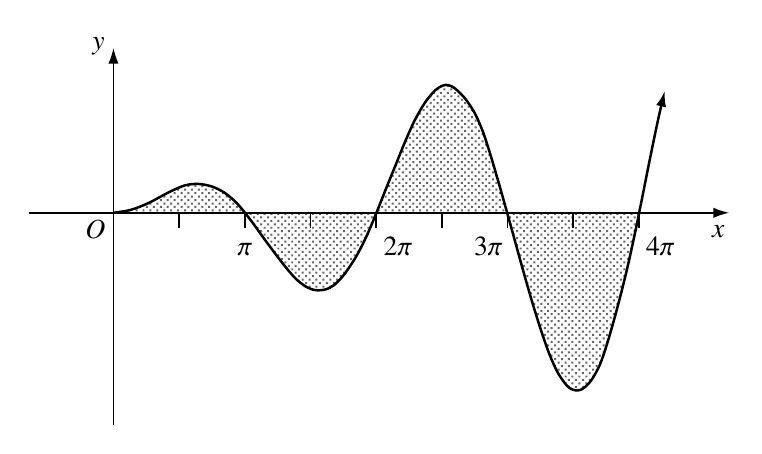
\begin{tikzpicture}[x=0.0127cm, y=-0.0127cm]
  \fill[shade dots, stipple color=black!60] plot[smooth] coordinates {(98,165) (114.1,162.4) (130.4,156.5) (148.5,147) (164.6,139.1) (176.9,136.3) (189.7,137.1) (202.7,141.3) (214.7,149) (226.9,160.9) (239,176.6) (252,195.9) (264.3,213.1) (276.7,226.8) (289.6,237.2) (299.8,242.3) (306.2,242.9) (313.3,240.2) (324.9,230.8) (336.1,217.9) (345.9,202.2) (354.5,183.9) (362.4,163.1) (370.4,141) (378.9,119.7) (388,98.27) (397.8,76.67) (406.7,58.48) (415.4,46.62) (423.6,40.08) (430,38.1) (436.8,39.09) (444.8,43.78) (452.4,52.83) (460.6,68.85) (468.8,88.7) (476.1,109.8) (482.7,131.9) (489.2,154.8) (495.6,178.2) (501.9,201.5) (508.4,224.8) (515,247.7) (521.8,270.2) (528.9,292.4) (536.2,312.2) (544.5,328.6) (551.7,338) (557.1,341.2) (563,341.6) (569.9,339.1) (576.3,333.2) (582.6,321.8) (589.8,301.9) (596.6,280.1) (602.8,257.8) (608.4,235.4) (613.6,212.2) (618.5,188.9) (623.5,165)} -- cycle;
  \draw[->] (13,165) -- (714,165);
  \draw[->] (98,377) -- (98,0);
  \foreach \k in {1,...,8} \draw ({98+65.7*\k},165) -- ({98+65.7*\k},180);
  \draw[->, line width=0.9pt] plot[smooth] coordinates {(98,165) (115.1,162.1) (132.7,155.4) (153.5,144.4) (169.4,137.6) (182.5,136.1) (196.2,138.6) (209.4,145.1) (222.1,156.1) (235.3,172.4) (250.6,193.5) (266.1,214.1) (279.6,230.2) (290.9,239.1) (300.2,242.4) (309.9,241.7) (318.6,237.4) (328.7,226.8) (340.4,209.4) (350.7,189.4) (360.3,166.9) (370,142.5) (380,117.9) (389.7,93.93) (399.5,72.2) (409.8,54.49) (419.9,42.36) (427.6,37.66) (432.7,37.26) (439.1,40.16) (449.7,50.56) (459.5,65.47) (467.7,84.17) (475.2,107.2) (482.6,132.3) (489.8,157.7) (496.9,183.2) (503.9,208.7) (511,234) (518.3,259) (526.1,283.7) (534.2,306.7) (542.5,325) (551.5,337.8) (557.4,341.9) (563,342.6) (568.3,340.5) (575.9,332.7) (584.3,317.7) (591.3,297.7) (598.6,272.7) (605.2,247.9) (611.4,222.9) (617.1,197.5) (622.5,171.8) (627.7,146) (632.9,119.9) (638.2,93.79) (643.6,68.35) (649.5,43)};
  \node[anchor=base] at (229.5,207.5) {$\pi$};
  \node[anchor=base] at (382.5,207.5) {$2\pi$};
  \node[anchor=base] at (473,207.5) {$3\pi$};
  \node[anchor=base] at (645,207.5) {$4\pi$};
  \node at (80,182) {$O$};
  \node at (702.5,184) {$x$};
  \node at (83,-2) {$y$};
\end{tikzpicture}
\end{document}
